%************************************************
\chapter{Evaluation \& Discussion}\label{ch:evaluation}
%************************************************
Our objective with this project was to design and implement an open-source simulation framework that can help developers of mobile context-aware systems to explore design alternatives. The framework was to dynamically classify physical objects, virtual objects and mediators that are close to the human agent according to the situative space model, with the human agent represented as an avatar that can move around and perform basic interaction with objects in the simulated environment.\\

In Section \ref{subsec:user_roles} we have identified three User Roles for the EgoSim framework. To evaluate to what extent we have met the goals defined in Section \ref{sec:goal}, we conducted an evaluation in two parts. First we have evaluated a simulation created with the EgoSim framework from the simulation user's perspective. The users were able to explore a ready made simulation while observing contextual changes in the context client. Second, we have evaluated the EgoSim framework from the system designer's perspective. The users had to build a simulation using our framework.\\

% For a complete assessment of the framework, we should have covered the third role as well, evaluating the system from a third party system's point of view. Normally, we would have asked the participants to build a piece of software which connect to our API and implements some business login on top of the retrieved data. Instead, to reduce the evaluation time, in the second evaluation step we gathered feedback about the API from the participants point of view. Moreover, we provided a task the where the participants had to 
%************************************************
\section{Participants} % (fold)
\label{sec:eval_participants}
%************************************************
In order to collect relevant technical feedback, we have aimed at recruiting participant having a fair amount of experience in software development. We have recruited a total of 17 participants. 15 of them are Software Engineers, 1 Post-Doctoral Researcher and 1 Associate Professor. In the beginning of the study they were asked to assess their experience in software engineering and, particularly, in mobile development. Moreover, we gathered information on their experience with context-aware computing and the egocentric interaction paradigm. We briefly present the statistics of our participants profile bellow:
\begin{itemize}
	\item Years of experience in Software Engineering -- an average of 6.41 (ranging from 3 - 15)
	\item Years of experience in Mobile Development -- an average of 1.56 (ranging from 0 - 5)
	\item Familiar with concepts Context-Aware Computing -- Yes: 47.1\% (8), No: 52.9\% (9)
	\item Has worked on context-aware system (e.g. a mobile APP using the device's location to perform implicit actions) -- Yes: 29.4\% (5), No: 70.6\% (12)
	\item Familiar with the egocentric interaction paradigm or the SSM -- Yes: 5.9\% (1), No: 94.1\% (16)
\end{itemize}

Analysing the profile of our participants, we can deduct that they have a good seniority level in software engineering and a fairly good knowledge of mobile development concepts. Almost non of them were aware of the egocentric interaction paradigm, but we were able to easily explain the concepts. Learning about the egocentric-interaction paradigm was made easy due to the vast experience the participants have in the field of software engineering.
% section sec:eval_participants (end)
%************************************************
\section{Procedure} % (fold)
\label{sec:eval_procedure}
%************************************************
We have developed a web page the participants were able access, read through the introduction to get up to speed with the terminology and where they could find the scenarios and tasks to finish the evaluation, as well as the feedback forms to help them get back to us with answers. This documentation can be accessed live on the project's evaluation web page \cite{evaluation:online} or in raw format in the source code repository \cite{evaluation:src}.\\

Going through the introduction, the participants were first introduced to concepts of context-aware computing, followed by an introduction to the egocentric-interaction paradigm and the situative space model. In the last part of the introduction we have presented the goals of our work and the features of the EgoSim framework.\\

Next, the participants were given three scenarios. The first step was the WarmUp task, meant to make the participant familiar with the simulator's concepts and ways of interacting with the environment. This step did not require any feedback. The WarmUp task is detailed in Section \ref{sec:eval_warmup_scenario}.\\

% In the second scenario we have developed a simulation for an Assisted Living Facility where objects around the human agent are categorised according to the SSM. For this scenario we have imagined the hypothetical situation where such a facility must be implemented.\\

% An ALF is a housing facility for people with disabilities. These facilities provide supervision or assistance with activities of daily living (ADLs) and monitoring of resident activities to help ensure their health, safety, and well-being. Basic ADLs consist of self-care tasks, including: dressing, eating and feeding, bathing and showering etc. Constantly monitoring and predicting the activities of ALF residents is imperative for software services in the ALF.\\

In the second scenario we have developed a simulation for an Assisted Living Facility where objects around the human agent are categorised according to the SSM. For this task the participants have evaluated the system from the simulation user's point of view. They had to test a ready made simulation with the EgoSim framework. The second task is detailed in Section \ref{sec:eval_alf_scenario}. In Figure \ref{fig:eval_alf_tryout} a participant is evaluating the ALF simulation.\\
\begin{figure}[H]
	\centering
	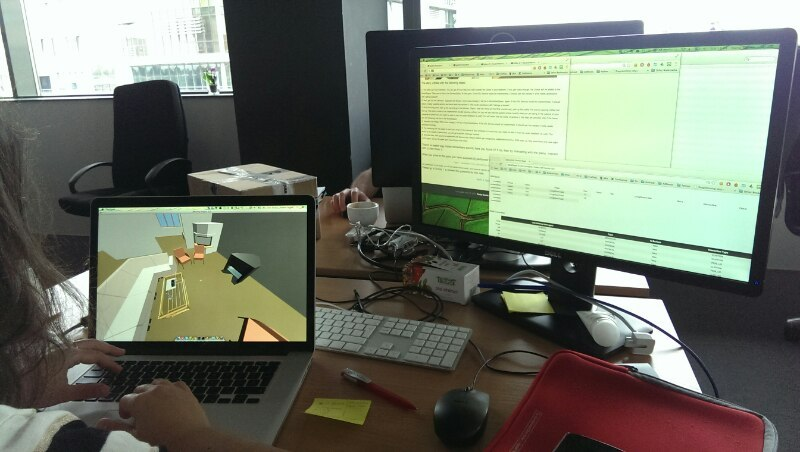
\includegraphics[width=\linewidth]{gfx/Chapter5/alf}
	\caption{A participant in our user-testing trying out the Assisted Living Facility Scenario}
	\label{fig:eval_alf_tryout}
\end{figure}

In the third scenario, the participants had to develop a new simulation using the EgoSim framework. The hypothetical problem they were given as part of this task is that families cannot make their homes secure enough for their children. Therefore, the participants were asked to imagine themselves being a system designer solving this problem using the EgoSim framework. This third task is detailed in Section \ref{sec:eval_childproof_scenario}. Setting up 3D models for EgoSim is done in third party software, therefore is out of scope for its evaluation. We have provided all the 3D models needed by the participants to finalize the tasks. In Figure \ref{fig:eval_childproof_tryout} a participant is using EgoSim to build the Childproof simulation.\\
\begin{figure}[H]
	\centering
	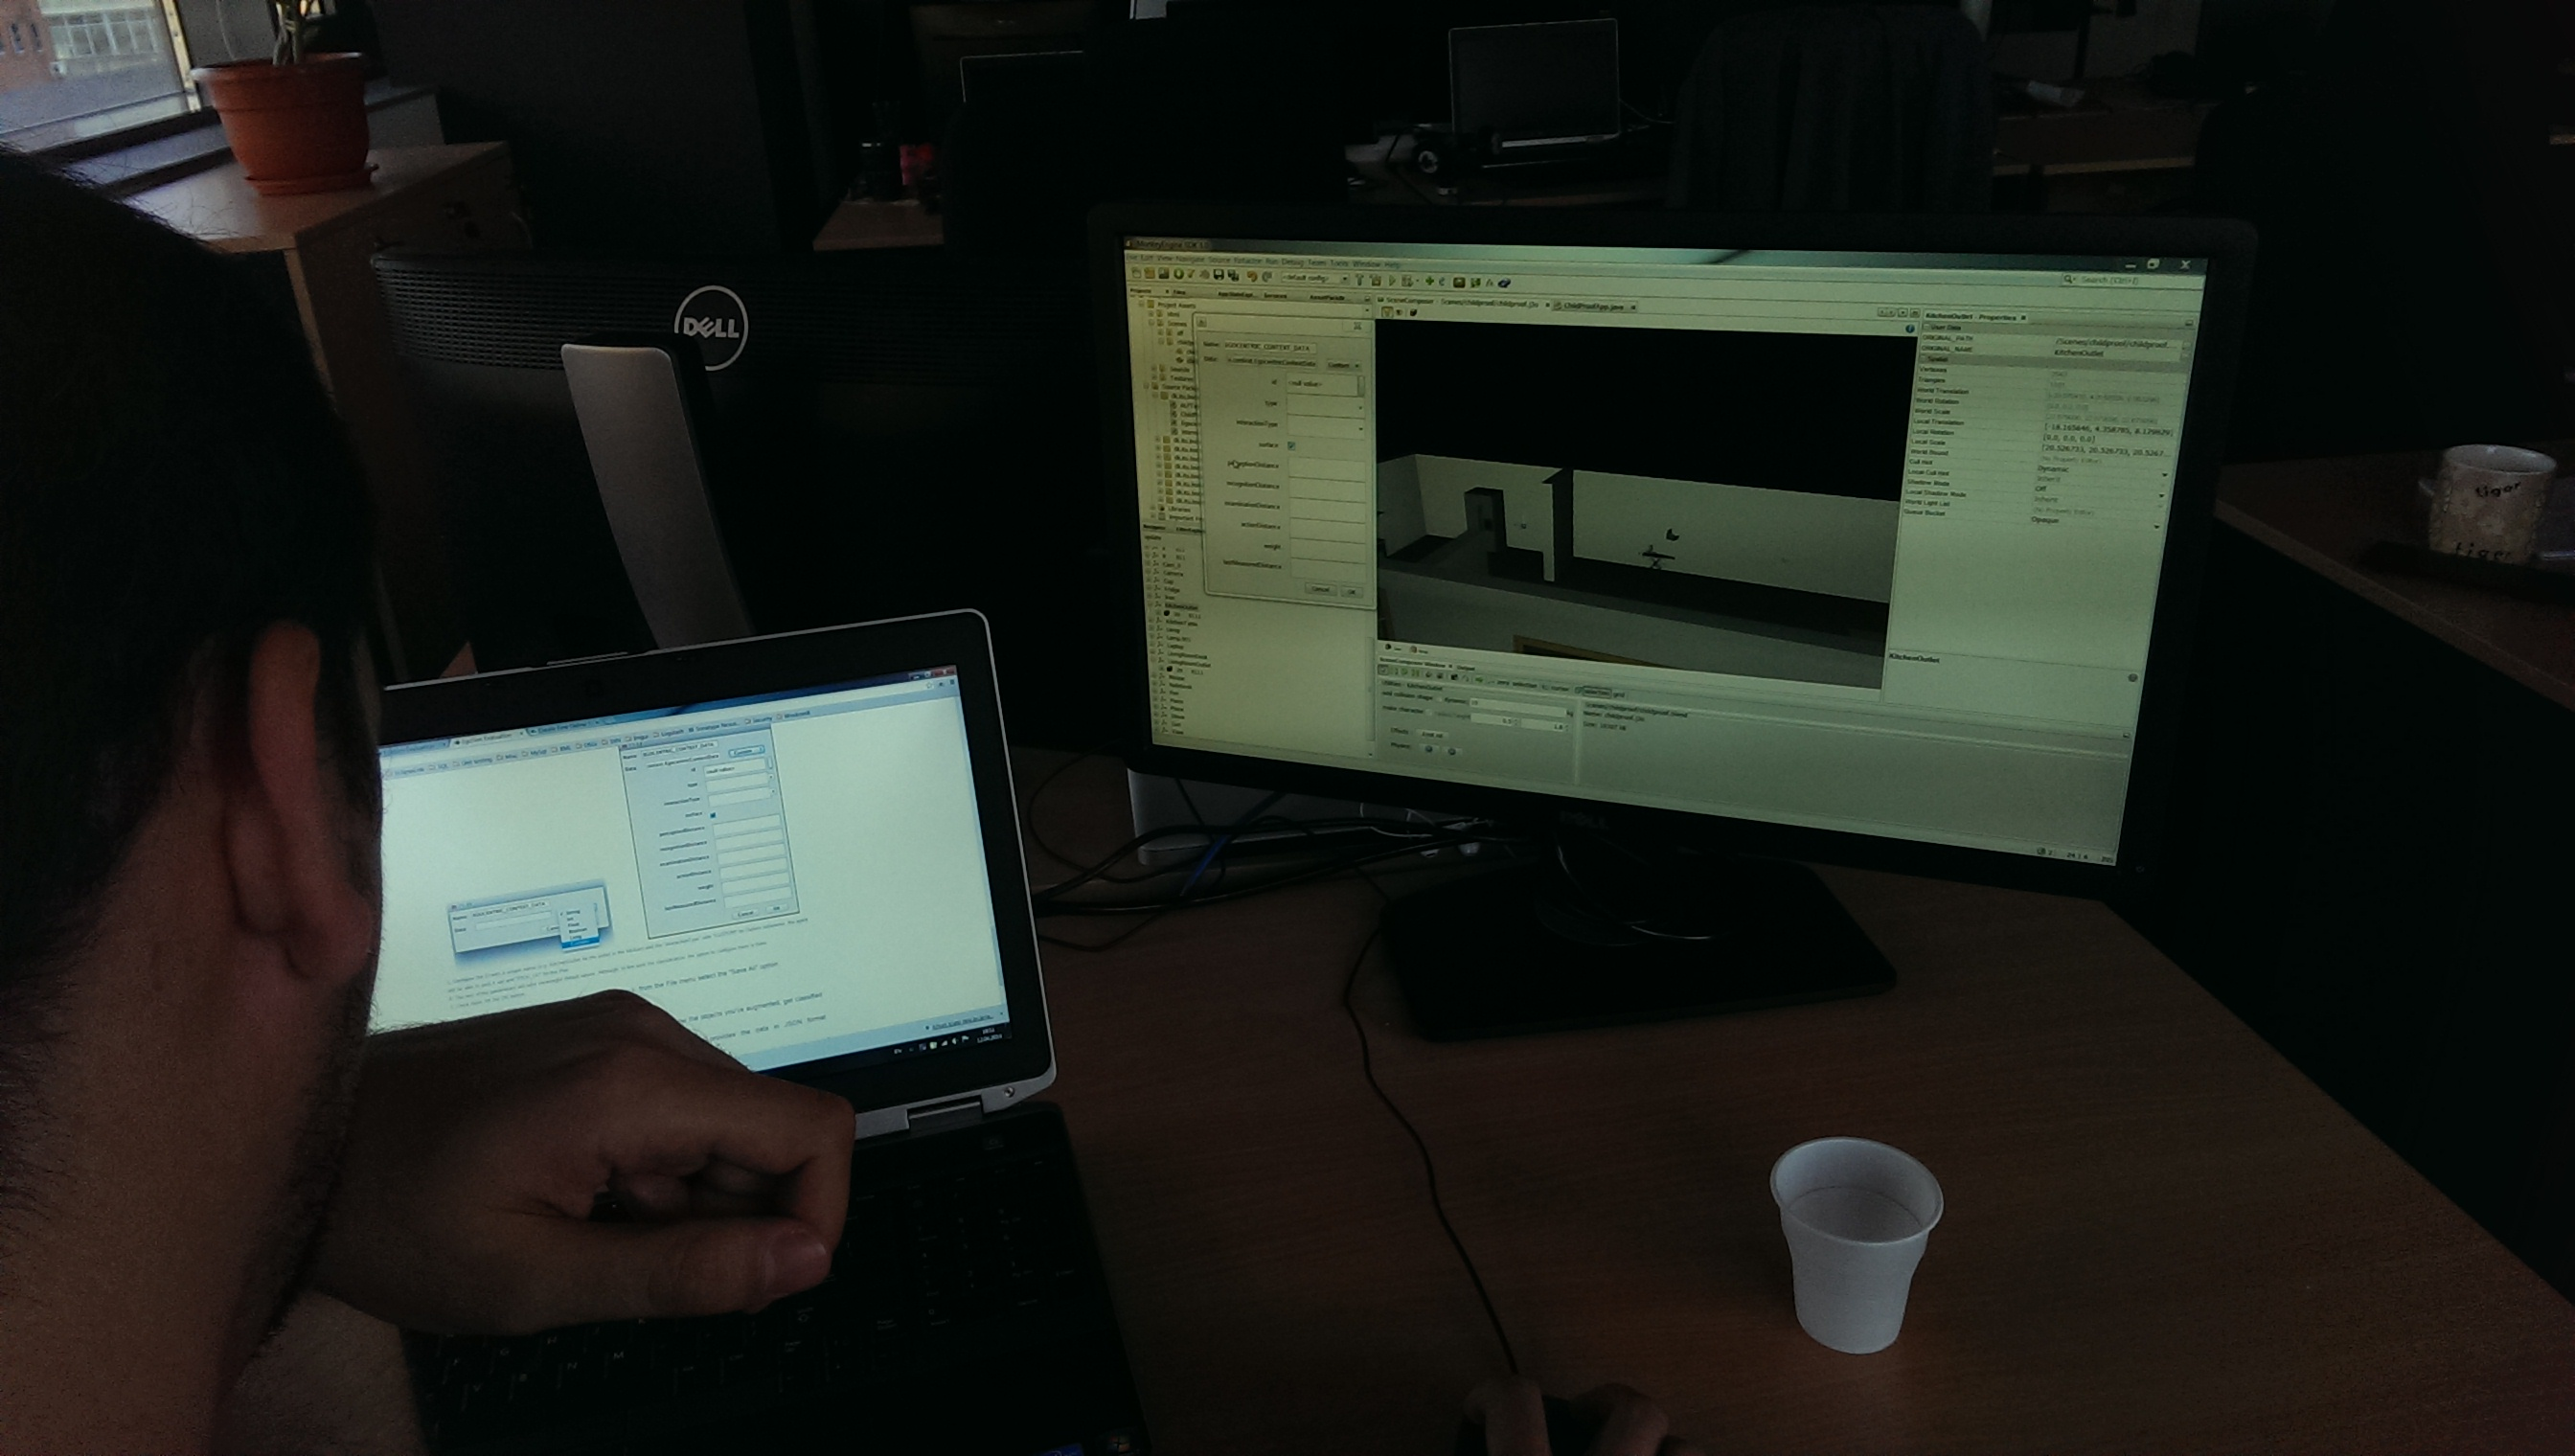
\includegraphics[width=\linewidth]{gfx/Chapter5/childproof}
	\caption{A participant in our user-testing building the simulation for the Childproof scenario}
	\label{fig:eval_childproof_tryout}
\end{figure}

Except for the warmup task, the participants were asked to fill in the feedback forms provided at the end of each evaluation scenario. The forms resemble a semi-structured interview which include questions regarding the usefulness of the system, usability of the framework and of the resulting simulations. Being a semi-structured interview, we had some open questions encouraging the participants to provide any sort of feedback that came to their mind about the system (software bugs they might have found, what they liked, what they didn't, etc).\\

We would have liked to do a comparative study where the participants would create similar simulations using one of the systems presented in the related work chapter \ref{ch:related_work}. However, those systems do not support some of the features our system making it impossible to implement a replica of the same simulation. Moreover, the systems in the related work do not provide classification of objects around the agent according to the SSM, which makes the results of a comparison between a simulation built with EgoSim and one of the systems in the related work irrelevant. We therefore proceed with a user-test of our system with no comparison to other methods.\\

In the semi-structured feedback form we have asked the participants a series of questions. The first set of question was about aspects of simulations built with EgoSim, asked from the simulation user's perspective as enumerated in Section \ref{sec:res_alf_task}. The second set of question was about the framework itself asked from the perspective of a system designer, as enumerated in Section \ref{sec:res_childproof_task}.\\

For a complete assessment of the framework, we should have covered the third role as well, evaluating the system from a third party system's point of view. Normally, we would have asked the participants to build a piece of software which connects to our API and implements some business login on top of the retrieved data. Instead, to reduce the evaluation time, in the second set of questions we gathered feedback about the API from the participants. Moreover, in the last question the participants were asked to describe in plain words or pseudo-code language the business logic to solve a given problem using the SSM Sets available through the API.\\

The whole evaluation session, including reading the documentation and providing feedback, lasted between 90 and 120 minutes.\\

Next, in Section \ref{sec:eval_discussion} we discuss the results of the evaluation and in Section \ref{sec:eval_future_work} we present our goals for future work.\\
% section sec:eval_procedure (end)
%************************************************
\section{Discussion} % (fold)
\label{sec:eval_discussion}
%************************************************
% The tool we have built is meant to be used by system designers to create simulations. The resulting systems are then used by simulation users and third party services. To meaningfully assess the quality of the EgoSim framework and of the simulations which can be built with it, we have to take a step back to inspect the goals \ref{sec:goal} and and requirements \ref{sec:requirements}. The requirements have been identified based on the goals of the system and guided by an end-to-end scenario \ref{sec:scenario} we have imagined as the intended way to use our system. Given that the result of our work is an interactive system, we have evaluated the system from the end user's point of view.\\

% To quantify the user feedback into a meaningful discussion, we have extracted four characteristics of interest which emerged from the goals and requirements of our system. For the system designer we wanted to create a framework which allows ''researchers to easily build a simulated environment''\ref{goal:1}, as detailed in requirements \ref{us:1} - \ref{us:3}. Within the simulations built by system designers, we wanted to allow simulation users to control a virtual agent in order to interact ''with the environment (move around, look around, pick up objects, etc)'' \ref{goal:2} (detailed in requirement \ref{us:4}). To evaluate how useful these requirements are and to what extent our system have met them, we will look into the \emph{usefulness} and \emph{usability} of both the framework and simulations from the end user's point of view.\\

% The simulation users interact with a visual heavy 

The evaluation results can be found in Appendix \ref{sec:res_alf_task} and Appendix \ref{sec:res_childproof_task}. Before we carry on with the discussion, we would like to point out one more time that the level of experience in the field of software engineering of all of our participants was high. We believe that the results of the evaluation provide good guidelines for future work on the system.\\

For the ALF evaluation scenario we came up with a hypothetical problem and provided a solution based on the SSM. We were concerned that the participants might not agree that designing the solution based on the egocentric interaction paradigm is the right approach. Therefore, we have asked them \ref{question1:6} whether the SSM is the right context model for the ALF system and for the third party services developed around it. All the participants agreed that this was the right approach, assuring that we have chosen a strong and relevant scenario for this evaluation.\\

%************************************************
\subsection{Usefulness} % (fold)
\label{sec:eval_usefulness}
%************************************************
One of the main objectives of our evaluation was to investigate if the users found our system useful. On one hand we were interested if the participants found simulations built using EgoSim as being useful; on the other hand if they have found the system as a whole useful to simulate system designed around the SSM context model.\\

All the participants have seen the value of simulating a system using EgoSim, over directly implementing the system into a real set-up. This strengthens the hypothesis of our work, that there is a real need for the system we have built. As one of the users stated in the feedback for question \ref{question1:7}: ''The simulation could provide a cost effective way of gaining valuable insight into the design of an Assisted Living Facility before such a facility is constructed''. Moreover, some participants pointed out some benefits of the simulator we have not stated:
\begin{itemize}
	\item lower costs in case of trial and error
	\item gives you a perception of how people interact with the objects
	\item faster feedback loop
	\item a simulation is a reliable and cheap proof of concept
	\item it allows the discovery of edge cases
\end{itemize}

To further assess the usefulness of EgoSim, all the users found it useful to simulate systems build with the SSM context model at their core. One of the participants stated in the feedback for question \ref{question2:2} ''Objects can be easily decorated with context information and interacting with them can be tested quickly because the framework takes care of basic interaction and movement in the space''. The fact that we have inferred functionality from based on the Ego Metadata configuration, makes the framework a lot more useful for users than we though in the first place. None but one of the participants were previously aware of the SSM context model, but they have managed to successfully build a simulation in the second task: ''with a few easy steps I was able to model the desired environment''.\\

When creating a simulation of a real life environment, immersion of the user into the virtual environment is rather important. The user must identify herself/himself with the agent and the simulated environment must resemble the real environment it actually represents. This has two implications: on one hand the 3D model of the environment must be good enough to resemble the real life setup of the simulated environment; on the other hand, the when the simulation is running and the user is interacting with the environment, she/he must feel absorbed to a certain extent. All the participants found the ALF simulation a good simulation for a home \ref{question1:1}. We have build both the ALF and the Childproof 3D models with a third party software and used them with our framework. Moreover, the participants have experienced the virtual environment by means of the running simulation. The fact that all participants found it a good simulation of a home, assures that third party software can supply useful 3D models. The feedback from our participants makes us believe that we made the right decision to use a game engine to render the 3D models and provide interaction capabilities.\\

We believed the level of object details for this evaluation was not relevant. One of the participants proved us wrong saying ''given the high system requirements I would have expected a better graphics/game engine''. Reflecting upon the issues this is not a game engine problem. The jMonkey Engine has all the capabilities of rendering high quality models. We have simply implemented models with low details. However, developing high detail models requires much more time invested in the modelling process.\\

Our system proved to be a useful educational tool as well. Before staring the evaluation, only one participants reported as being familiar with the egocentric interaction paradigm \ref{question1:0}. After the evaluation the participants have reported an average of 4.5 level of understanding about the SSM, on a scale from 1 to 7 \ref{question2:0}. This means using the EgoSim framework, participants got rather good insights into what egocentric integration paradigm means and how the SSM works. In the future, it might prove to be a useful tool for students studying ubiquitous computing to learn about these concepts.\\

In one of the feedback questions we have asked the participants to imagine various system they could build using based on the SSM Sets and the outcome of our classification algorithms. The have came up with a list of interesting ideas \ref{question2:10}; we have listed some of them bellow:
\begin{itemize}
	\item Assistance for people with disabilities (especially the visually impaired), to offer a augmented representation of their environment.
	\item A tourist map that is context aware and can recommend places to visit that are near the current location, that are for example still open (maybe it's night, you don't want recommendations for a zoo), etc.
	\item Security application: auto-lock my computer screen when it is in my Action Space.
	\item Automatic light switching based on the position of the inhabitant of a home (not motion-based). This can be generalized to a system that defines custom operation modes of devices in a home, depending on what the user is doing.
\end{itemize}

All of these systems/services are useful systems and they can easily be simulated with EgoSim. The fact that so many participants were able to come up with ideas of systems build on top of the SSM context model, means the context model has a lot of potential for context aware system development. Therefore, the support EgoSim offers for building simulations with this context model as a cornerstone, based on the user feedback, turns out to be useful based on the user feedback.
% section sec:eval_usefulness (end)

%************************************************
\subsection{Usability} % (fold)
\label{sec:eval_usability}
%************************************************
All participants were positive about the usability of the system. Creating a simulation using EgoSim comes down to do some configuration work on top of a 3D model. Using EgoSim to design a new simulations, the participants have reported that identifying and configuring the objects to be classified during simulation, on a scale from 1 to 7 (Very easy - Very hard) was an average of 2.1 \ref{question2:3}. This means that almost everyone has found the process of designing a new simulation easy. We have based this process on the jMonkey SDK's components. We were sceptical at first and thought it might be a laborious and hard to understand process, but based on the user feedback, we conclude it was the right decision.\\

Although, one of the participants was not able to finish the second task \ref{question2:1} because due to not being able to augment the desired object models with EgocentricContextData. This was most probably due to the fact that when configuring an object in the jMonkey scene composer, the name of the custom user data must be EGOCENTRIC\_CONTEXT\_DATA. If it is not exactly this, even if the name has an extra space, the framework will fail to identify object to be classified. A user feedback to improve this feature was to ''trim the context variable for space EGOCENTRIC\_CONTEXT\_DATA''. We could indeed rephrase the name into something shorter, but this is a matter for future work.\\

When running the simulation, the participants felt that interacting with the environment was very intuitive. On a scale from 1 to 7 (Not intuitive at all -- Highly intuitive), they have reported an average of 5.5 \ref{question1:3}. This translates into the interaction with the environment being very intuitive. This is of course valid only for moving around the environment and for the default interaction we have provided for objects -- pick-up/drop-down. Some users felt that a generic USE action would be more appropriate ''A generic USE action would help is many situations as many objects that are interacted with might have a main USE method. pickup/putdown could be specific implementations of use''. Moreover, other kind of interactions have been requests like turn off/on for electronics, shower, etc. All these aspects will be discussed in Section \ref{sec:future_work}.\\

The collision detection (the fact the agent could not pass through objects) was especially well received ''I think moving around was very close to reality and I liked the fact that it was aware of the obstacles. For example, you could not just move forward through the couch to get to the coffee table''.\\

The custom interactions we have implemented in the fist scenario were also well received: ''The Piano playing actions were nice''. Some participants noted that support for building custom interaction would have been useful: ''Would be nice if people could declare their own type of interactions''. This is actually possible with the current implementation, unfortunately we could not fit any more tasks for the participants in the evaluation; it took a fair amount of time as it is. The fact that it is a required feature, means we have well anticipated this need by implementing support for both CUSTOM interaction with objects, as detailed in Listing \ref{lst:custom_interaction}, and COMBINED interaction between two objects, as detailed in Listing \ref{lst:custom_interaction}.\\

Most context aware systems need to access the historical information of changes in context of various entities. We have not implemented this aspect, but we should plan for this in future work. On of the participants even mentioned the lack of this feature stating that it would be useful to have ''Historical information about the agent: what actions has he performed so far, objects with which he has interacted with so far, etc''.\\

To evaluate the framework from a third party service's point of view, in the second task we have given the participants to solve a hypothetical problem in the context of the scenario, as a developer of a third party service based on data available through the API. 16 out of the 17 participants were able to provide the correct solution \ref{question2:10}. This makes us believe the data in the SSM sets provided through the API is explicit enough to build service aware of the current context in the ongoing simulation.\\

In the current implementation context changes occur only as the agent interacts with the environment. Some participants pointed out that it would be useful to modify some context data through the API. We will reconsider this idea in future work.\\

A potential weakness of the framework was pointed out by one of the participants saying ''a potential weakness of this framework would be the lack of information regarding the relationship between objects''. In the current implementation we monitor the context of surrounding object only from the agent's perspective. But context information that is affected by relationship between objects might also be relevant. This could be solved by adding support for sensor to our framework, which we lack at the moment.\\

Overall, the framework as a whole was perceive by the participants as being highly useful \ref{question2:3}. One of the participants even said that ''it is very easy to import a scene and augment the objects with different information and interaction types''.\\
% section sec:eval_usability (end)

%************************************************
\subsection{Responsiveness} % (fold)
\label{sec:eval_responsiveness}
%************************************************
Target of our evaluation was also to assess how responsive the simulation and the context client turned out to be. The simulation was found to be responsive and running smoothly by 88.2\% of the participants \ref{question1:8}. We are especially happy about this outcome because the classification process implies heavy computation under the hood, which means we have done the right thing implementing the classification as a standalone process. One of the users reported that ''there was a glitch when I could not move forward when getting out of bed. I had to move in a different direction and after that come back and approach the closet''. This is most probably because we have used a deprecated CharacterControl\footnote{\url{http://hub.jmonkeyengine.org/javadoc/com/jme3/bullet/control/CharacterControl.html}} class from the jMonkey framework to help us in with the agent's movement. In future work we should address this issues by upgrading to the BetterCharacterControl\footnote{\url{http://hub.jmonkeyengine.org/javadoc/com/jme3/bullet/control/BetterCharacterControl.html}} class.\\

When asked about the responsiveness of the context client \ref{question1:5}, 76.5\% of the participants reported it being responsive and updating the context changes close to real time. Some comment from the other 23.5\% made us realised that there's place for improvement for the context client. Currently the context client is implement as a web page served from within the running simulation. The page automatically updates every second. This approach has some drawbacks as it will not display the context changes instantaneously. Moreover, it queries all the SSM sets over and over again without some of them modifying at all. This creates an unnecessary overhead as the context client is accessing the same shared resource the API and classification modules are using. Therefore, a more suitable implementation for the context client would be based on web sockets. This way, we would reverse the flow of information; the server would send notifications to the opened web page every time a change in context occurs. Anyhow, for the purpose of this evaluation, the context client played out well, and it's responsiveness was well received.
% section sec:eval_responsiveness (end)

%************************************************
\subsection{Classification} % (fold)
\label{sec:eval_classification}
%************************************************
A little more than half of the users have reported that the monitored objects were correctly classified into SSM sets \ref{question1:2}. This means our classification algorithm performed decently. The rest of the participants reported there were cases when the classification did not work as expected. There were two problems the users have noticed which prevented the classification to work as expected.\\

The first problem was that some objects were not being classified at all. These objects were actually never augmented with egocentric data, therefore with the current implementation, the cannot be classified. We though this was clear from the description in the evaluation, but we might have had to stress more on this matter. However, is all the objects in a scene were to be augmented with Ego metadata, during simulation they would all be taken into account and classified.\\

The second problem was that although some objects were visible, they were not classified as being perceived by the agent. This is a problem we are aware of and plan on addressing in future work. At the heart of our classification algorithm lies the way we determine if an object is currently visible to the agent or not. To do this, we cast a ray from the agent's current location to the centre point of the object's bounding box (think of it a the object's centre of gravity). If the ray intersects any other object before hitting the middle of the object, we consider the object as not being visible to the agent. This work in most cases, as the user feedback shows. But it has a lot of edge cases. For example the centre of a table can be occluded by a coin; this does not make the table unrecognisable, it just make our algorithm generate a false positive. Likewise, the agent could see through a hole in the wall the only centre of a drawer. Without other details, that object might be unrecognisable.\\

One of the participants provided a very helpful feedback in this matter ''I consider the condition for an object to enter the perception space to be too weak. A user cannot identify an object if only a pixel is within his field of vision. Humans are built to recognize patterns, therefore a pattern-oriented metric could be used. For instance, the introduction of a diversity factor would help the simulation. If enough diversity of the object is within the perception space, it could trigger its presence in the perception space''. We entirely share this opinion and will be taken into consideration in further improvements of the classification algorithm.\\

For the agent to be able to interact with an object, that objects must be in the ActionSpace, therefore within reach, or within the ActionDistance. We have tailored default value for this property. The system designer is free to modify this value at design time, but the participants did not modify it. Most of them (88.2\%) have felt that the default value was close to realistic \ref{question1:2}. One participant felt it was too close and another that it was too far. The problem discussed above has impact when classifying into each sets, therefore affecting the interaction between the agent and the surrounding objects.\\

Taking a step back to Section \ref{sec:eval_usability}, the fact that such a large number of participants have found interacting with the surrounding objects highly intuitive, means that they were able to easily pickup/drop down objects. This means the classifications are running close to real time. Why is that? Because every time the field of vision of the agent changes, we run a new classification. Even the slightest change to user's field of vision would trigger a new classification. Within the framework, decision are taken based on the latest available result of the classifications. As the simulation was perceived to run smoothly and interacting with the environment seemed natural, we conclude that decisions during the simulation were made according to the current context, meaning the classifications were execute almost instantaneously. In future work it would be interesting to evaluate how a very large number of tracked objects affect the performance of our classification algorithm.
% section sec:eval_classification (end)

% section sec:eval_discussion (end)
%************************************************
\section{Future Work} % (fold)
\label{sec:eval_future_work}
%************************************************
We have received a fair amount of feedback from our participants, as detailed in Chapter \ref{ch:evaluation_results}. We have collected all this user feedback into issues and enhancements in our source code repository \cite{issues:online}. GitHub\footnote{\url{https://github.com/}}, the hosting service we use for our source code repository, offers the ''issues'' feature. This way issues can be managed on the same repository we keep our code in. Being open source, if anyone is willing to contribute to the project, immediate work items are already created and can be addressed.\\

In the remaining of this section we will detail the proposed future development for the EgoSim framework. Some of the proposed ideas were mentioned in previous sections of this thesis, others come from the user feedback.\\

\paragraph{Interaction with virtual objects.} We have taken the compromise to limit the current implementation to physical objects and devices. But to fully support the SSM context model, virtual objects must be classified as well. A virtual object can be a window displayed on display, or a song played on a mobile device. Interaction with these objects is done through mediators (devices).

\paragraph{Third-person perspective.} Avatar based games and simulations usually provide both first-person and third-person views, with an easy way to switch perspectives during runtime. For this project, a third-person perspective could be useful if we are to represent wearable devices. Also, it would the simulation user to observe the various body gestures the agent is doing. Moreover, in a third-person perspective the simulation user could get a better understanding of the agent's immediate surroundings.

\paragraph{Improve detection of objects in the agent's field of view.} At the heart of our classification algorithm lies the way we determine if an object is currently visible to the agent or not. To do this, we cast
a ray from the agent's current location to the centre point of the object's bounding box (think of it a the object's centre of gravity). If the ray intersects any other object before hitting the middle of the object,
we consider the object as not being visible to the agent. This work in most cases, as the user feedback shows. But it has a lot of edge cases. For example the centre of a table can be occluded by a coin; this does not make the table unrecognisable, it just make our algorithm generate a false positive. Likewise, the agent could see through a hole in the wall the only centre of a drawer. Without other details, that object
might be unrecognisable.\\

One of the participants provided a very helpful feedback in this matter ''I consider the condition for an object to enter the perception space to be too weak. A user cannot identify an object if only a pixel is within his field of vision. Humans are built to recognize patterns, therefore a pattern-oriented metric could be used. For instance, the introduction of a diversity factor would help the simulation. If enough diversity of the object is within the perception space, it could trigger its presence in the perception space''. We entirely share this opinion and we will look into improving the classification algorithm as such.

\paragraph{Improve computation of distance to objects.} When computing the distance to a certain object, we measure the distance from the agent's current location to the centre point of the object's bounding box. Therefore the distance might not always seem accurate because we are not taking into consideration the shape of the object. A possible solution would be to cast a ray from the agent's location to the centre of the object's bounding box and compute the distance to the closest intersection point (where the ray intersects the object). This way we could obtain a more accurate distance.

\paragraph{A more granular perception of entities.} In the current implementation we have used a less generic definition of the SSM spaces. Future work could broaden them up to provide a classification closer to the ones defined in the theoretical framework. For example, an object in the Perception Space can be perceived as different entities depending on the distance to the agent. Given a hammer, from the furthest perception distance (X1) the agent would perceive it as an object; from a closer distance (X2), the agent would perceive it as an object certain kind of shape while from a more closer distance (X3), the agent would perceive it as hammer. So, an object should be perceived in different ways based on the agent's proximity.

\paragraph{Improved API.} In this implementation to retrieve data from the API a third party service has to query the endpoint every time it need updated data. This creates unnecessary overhead both for the framework and for the service. To improve this, we plan to look into alternatives, for instance an API based on publish/subscribe. With this communication pattern we would allow service to express their interest in contextual changes based on some rules they define. For example context changes of a certain entity with a given ID, context changes within a certain set, etc. Whenever one of the registered events occurs, the API would broadcast the event and every service registered for that type of event would receive the notification. With this pattern we can minimize the overhead on both the API's and the third party service's side. Moreover, the delivery of the notification would happen real-time, the service being able to take action at the same moment a certain context change has occurred.\\

We are also interested in evaluating if there would be value for third party service to dynamically manipulate some attribute through the API. For example, an external service might automatically turn up the light if the agent walks into a certain room.

\paragraph{Improved ContextClient.} The advantage of having implemented the context client as a web page, is that no additional software installation is required. It can be accessed from any browser, on any platform. The problem with the current implementation is that it does not reflect the new information immediately after a change in the context occurs. It only does so every second. To improve refresh time, we though of using Web Sockets\footnote{\url{http://www.websocket.org}}. The WebSocket specification defines a full-duplex single socket connection over which messages can be sent between client and server. This means that instead of refreshing the context client every second, the ContextViewServer could push up to date information towards the context client, whenever available, through an open web socket connection.

\paragraph{Improved context information.} Many participants have pointed out that more context data should be monitored, besides visibility and proximity. To mention some of them: temperature, on/off state, orientation of certain objects (i.e. a computer screen might be close but you might be viewing it from behind), etc. We agree that for a complete context aware system some of these attributes have to be monitored by the framework. Another attribute useful context information we are interested in monitoring is the distance between objects. At the moment we only monitor the distance of objects relative to the agent's position. Knowing the distance between certain objects might be an important information for building business logic. Of course, adding more context information means to have it available through the API as well.\\

\paragraph{Evaluate how a very large number of tracked objects affect the performance of our classification algorithm.} During the evaluation process we have built a couple of simulations using the EgoSim framework. Within a simulation we have tracked around 20 objects at a time. With this number of tracked objects, the simulations ran smoothly providing up to date SSM sets throughout the lifetime of the simulation. We plan on setting up a simulation where we monitor a large number of objects to see how that affects the performance of the classification algorithms, hence the simulation overall. We think there should not be much of a difference as we only take into account the objects currently in the agents field of vision which are usually constant in number through the lifetime of a simulation. But we leave this conclusion to be drawn once this research has been conducted in future work.

\paragraph{Improved interaction between the agent and the environment.} We have received some interesting improvement ideas from the user feedback. To give a better feedback for the simulation user, we might display a relevant icon when the agent is targeting a certain objects which is in the ActionSpace to denote that the object can be interacted with. This enhancement could improve the simulation user's experience.\\

Next, we are interested designing a generic USE action when interacting with objects. Therefore, instead of taking a default action when the agent tries to interact with an objects, the simulation could display a list of actions available for that specific object; the list of actions would depend on the current context. For example, trying to interact with a mobile device could provide two actions: \emph{pick-up} and \emph{interact}. The \emph{pick-up} action would simply pick the object object up, while the \emph{interact} action would allow interacting with the virtual objects within the mobile device.\\

In this version of the framework the only default action we have provided is pick-up/drop-down. Some of the participants have mentioned other useful default actions like pull/push for drawers, open/close for doors, drop object at current location, turn on/off for switches, lamps, etc. All of these actions broaden the interactions the agent is enable do with the environment. We will plan on implementing these default actions.\\

In the current implementation we have used a deprecated CharacterControl\footnote{\url{http://hub.jmonkeyengine.org/javadoc/com/jme3/bullet/control/
CharacterControl.html}} class from the jMonkey framework to help us in with the agent's movement. As the CharacterControll class became deprecated, we plan on upgrading to the BetterCharacterControl\footnote{\url{http://hub.jmonkeyengine.org/javadoc/com/jme3/bullet/control/
BetterCharacterControl.html}} class. This will solve some of the agent navigation issues encountered during the evaluation process.

\paragraph{Integration with a Virtual Reality (VR) kit.} This is an idea we have got from one of the participants. Integrating the simulation with a VR kit would create allow for maximum immersion of the simulation user into the simulated environment. On such VR kit is the Oculus Rift\footnote{\url{http://www.oculusvr.com/}} VR kit. The community of jMonkey Engine has already made some advances in integrating it with the Oculus Rift SDK. We are really interested looking into this aspect in future work, as we believe it has to offer a lot of benefits for how the simulation user experiences the simulated environment.

\paragraph{Create an EgoSim IDE.} The jMonkey Engine SDK is free and open source. To create an integrated development experience for the system designer, we have the option extending the SDK and creating an EgoSim IDE of our own, making the configuration process easier and providing EgoSim specific design options. This would require a large amount of work. First because we need to dig deep into understanding how jMonkey Engine is implemented. Moreover, we need experience in developing plug-ins for the NetBeans platform, as the JME SDK is developed on top of NetBeans. At the moment this is not our biggest priority, but we are not excluding the possibility of looking into this aspect in the future.
% section sec:eval_future_work (end)
%************************************************
\section{Comparison to existing systems} % (fold)
\label{sec:eval_comparison}
%************************************************
We have designed and implemented a framework that allows system designers to create simulations of mobile context-aware systems. The simulator empowers users to intuitively interact with the simulated environment, while classifying the objects around the agent according to the SSM context model.\\

UbiWise \ref{sec:ubiwise} is a device-centric simulator, it focuses on user manipulation of devices and the
interactions between devices.\\

TATUS \ref{sec:tatus} targets the intelligent technology controlling ubiquitous computing environments through the use of embedded sensors and actuators.\\

In Section \ref{subsec:user_roles} we have identified three roles for the EgoSim system. For two of them we have found similar roles in all the systems from the relate work described in Chapter \ref{ch:related_work}: the system designer and the simulation user. Some systems might not have used the same terminology. For system designer some of the related work have used the term \emph{researcher}, while for the simulation user has been named in some related works simply as \emph{user}.\\

We conclude this chapter with a comparison on how some of the simulators presented in the related work differ from EgoSim, with respect to each of these roles. We have chosen only UbiWise and TATUS as their simulator are closest to ours, meaning that they represent the target environment as a 3D model. Moreover, they use a game engine to render the environment and to allow users to interact with it.

%************************************************
\subsection{Role1: The System Designer} % (fold)
\label{subsec:eval_role_system_designer}
%************************************************
The system designer is a researcher or a developer designing and implementing a simulation of a context-aware system. This role shares a common working methodology throughout all three systems:
\begin{enumerate}
	\item using an editor, she/he creates a 3D model of the simulate environment
	\item using the framework and the underlying game engine, she/he develops the simulation's business logic. This step might need thorough understanding of the game engine, in case the system designer has to implement more than what the framework has to offer
\end{enumerate}

%************************************************
\subsubsection{UbiWise} % (fold)
%************************************************
''The building blocks of UbiWise are the simulated devices, the virtual representations of the physical devices''\cite{barton2003ubiwise}. Using a designer written in Java, the system designer creates a model of the simulated device. This model will be represented both in the 2D and the 3D view. Next, the system designer uses GtkRadiant\footnote{\url{http://icculus.org/gtkradiant}} to design the 3D model of the simulated physical environment where the device will be used. GtkRadiant is the official level design tool chain for the Q3A game engine. The drawback of this environment designer, as stated in the UbiWise paper is ''Operation of this editor is complex and it takes a couple of days to understand it; online resources for models often require format conversions to work in the editor. Thus the effort for the first simulation could be a week's time;''\cite{barton2003ubiwise}. The last step is to provide functionality for the device. This is done by means of an XML configuration file. It configures various actions to be handled by custom Java classes. These actions will be triggered from the 2D view.\\

%************************************************
\subsubsection{TATUS} % (fold)
%************************************************
In TATUS, the system designer uses the Hammer\footnote{\url{https://developer.valvesoftware.com/wiki/Valve_Hammer_Editor}} map editor to model an environment. It is a drawing tool for building maps. Hammer compiles maps a format used by the Half-Life game engine, which TATUS was built upon. To add sensors/actuators to the environment, the system designer would place \emph{triggers} at various locations in the map. Triggers are specific concepts from the Half-Life game engine. For clarity, imagine them as invisible entities within a map, which generate events based on a player's movements and location. So, if a player enters a region of a map occupied by a trigger the associated event is activated (e.g. a door is opened).\\

Next, the TATUS framework handles the aggregation of the generated messages; basically manages the context of the simulation. The context information is available through an API. To develop the simulation's business logic, the system designer implements a new System Under Test (SUT), in Java, which connects to the API and implements business logic based on the available context information.\\

%************************************************
\subsubsection{EgoSim} % (fold)
%************************************************
For EgoSim, the system designer can use one of the many 3D modelling software to generate compatible 3D models with the underlying game engine, one of them being Blender\footnote{\url{http://www.blender.org/}}. The model can than be imported into the scene composer where the system designer identifies the objects he wants classified according to the SSM context model. To finalise the simulation, the system designer has to write some Java code by extending an abstraction provided by the framework. The abstraction will only need the model to use and some initial configuration data. If desired, the abstraction provide callback methods to implement functionality for custom interactions. During the simulation, the framework makes the context data available through an API available to third party services.\\

%************************************************
\subsubsection{Discussion} % (fold)
%************************************************
Because of the game engines they have used, developing the model of an environment for UbiWise or TATUS is bound to their specific map editors. EgoSim, on the other hand, is based on jMonkey Engine which works with various third party 3D model formats. We consider this being a plus. For example Blender, on of the software producing compatible formats, is the most popular open source 3D modelling software. The community produces a lot of free model which can be reused. Moreover, it is well documented which together with the active community helps a system designer get up to speed fairly quick.\\

If the system designer is in need to develop custom functionality and needs to go to the game engine level, TATUS and UbiWise impose quite a challenge. Both game engines were written in C/C++. As stated in TATUS ''Following the experiences encountered while working with the HL SDK, it has become apparent that its complexity requires the presence of an experienced developer. In order to tackle the SDK, a developer must at least have a good working knowledge of C/C++''. EgoSim on the other hand is based on jMonkey Engine. It is written in Java, a language widely embraced by the research community. Moreover, it's open source and well documented. A system designer experienced in Java should be able to get up to speed and become proactive within a few day with jMonkey Engine.\\
% section sec:eval_role_system_designer (end)

%************************************************
\subsection{Role2: The Simulation User} % (fold)
\label{subsec:eval_role_simulation_user}
%************************************************
This role is filled up by a person running a simulation build with one of the frameworks. In all three cases, the user interacts from a first-person view with the simulated environment.\\

%************************************************
\subsubsection{UbiWise} % (fold)
%************************************************
UbiWise offers two views to the user, the 3D physical view (game environment) and the 2D device view (Java Swing Interface). A user in such an instance does all manipulation of the devices through the device view only. The 3D view is used solely to see the effects of device manipulation on the 3D environment. For example, in the example scenario the agent carries a digital wireless camera and in the simulated environment there is a wireless picture frame, both connected to the same content service. When the user uploads a picture from the 2D view, the wireless picture frame reflects the picture that has been uploaded.\\

%************************************************
\subsubsection{TATUS} % (fold)
%************************************************
TATUS offers a 3D view. The simulation user can experience the physical environment fully immersed throughout the lifetime of the simulation. The environment will be modified by the SUT based on the business logic implemented for a specific situation (in a certain context). For example, if the agent is close enough to a door, the SUT might decide to open that door. Therefore, TATUS specifically targets predicting user intentions based on notifications from sensors and actuators embedded in the environment. The simulation user experiences changes in the environment while interacting with it, as effect of the SUT's business logic controlling the ubiquitous computing environments through the use of embedded sensors and actuators.\\

%************************************************
\subsubsection{EgoSim} % (fold)
%************************************************
EgoSim offers a 3D view. The simulation user can interact with the simulated environment by moving around and performing basic interactions with everyday objects (i.e. pick-up/drop-down). As the simulation unfolds, the underlying monitoring service classifies the objects in the agent's surroundings according to the SSM context model. This context information can be accessed from a third party service through an API. Applications build on top of this context model can be always aware of the agent's surroundings, being able to take appropriate actions. Moreover, the simulation user has access to a ContextClient which displays the current status of the SSM context model. This can be used to observe if the simulation was correctly set up.\\

%************************************************
\subsubsection{Discussion} % (fold)
%************************************************
In all cases the user interacts with a 3D environment, but each environment is meant for a certain type of interaction: UbiWise is device centric, TATUS is sensor centric while EgoSim is body centric.
% section sec:eval_role_simulation_user (end)

% section sec:eval_comparisond (end)
%************************************************
\section{Conclusion} % (fold)
\label{sec:eval_conclusion}
%************************************************
The results presented in this chapter, conclude that we have managed to develop a usable open-source simulation tool for applications designed based on the egocentric interaction paradigm. We have managed to satisfy the objectives laid out in Section \ref{sec:goal}. By fulfilling the current work we have successfully implemented a first version the EgoSim framework, with many possibilities for future work as detailed in Section \ref{sec:future_work}. The feedback from our evaluation participants have strengthened the assumption that there is a real need for this tool, as they have provided concrete examples of real-life problems solve using the SSM context model. Finally, the comparison between UbiWise, TATUS and EgoSim confirms that this framework contributes with another dimension to the worlds of 3D ubiquitous computing simulators.
% section sec:eval_conclusion (end)